\chapter{Computational aspects of Fluid-Structure Interaction problems}
\label{cha:computation}

This section deals with the computational aspects of FSI problems. The first possible categorization of solution techniques distinguishes between monolithic and partitioned approach, as discussed in Section \ref{sec:monolithic}. This work is based on the latter approach, so the two different coupling strategies, namely strong and weak, are discussed in Section \ref{sec:coupling}. As strong coupling is generally needed for accurate solution, ad overview of strong coupling algorithms is given in Section \ref{sec:strong-coupling}. Section \ref{sec:interface-mesh} focuses on aspects concerning the interface mesh, and how the solid and the fluid exchange data between them. Finally \ref{sec:added-mass} briefly describes a common issue arising in strongly coupled problems: the ~\ac{AME}.


\section{Monolithic and Partitioned Approach}
\label{sec:monolithic}

Analytical solutions are impossible to obtain for the large majority of FSI problems; on the other hand, laboratory experiments may be costly, unfeasible or limited. For those reasons, numerical simulations may be employed to analyze the physics involved in the interaction between fluids and solids. With the current capabilities of computer technology, simulations of scientific and engineering models have become increasingly detailed and sophisticated.

The numerical methods used to solve FSI problems may be roughly classified into two classes: the \textit{monolithic approach} and the \textit{partitioned approach}. There is no exact distinction between the two approaches, as they might be seen differently among fields of applications. The idea here is to consider how many solvers are used to find a solution.

In the \textit{monolithic approach}, the whole problem is treated as a unique entity and solved simultaneously with a specialized ad hoc solver (see Figure \ref{fig:monolithic}). The fluid and structure dynamics form a single system of equations for the entire problem, which is solved simultaneously by a unified algorithm. The interface conditions are implicit in the solution procedure \cite{hubner2004monolithic}, \cite{ryzhakov2010monolithic}.

This approach can potentially achieve better accuracy, as they solve the system of equations exactly the interface conditions are implicit in the model \cite{richter2017fluid}, but it may require more resources and expertise to develop from scratch a specialized code (it solves a very specific model) that can be cumbersome to maintain.

\begin{figure}[htbp!]
	\centering
	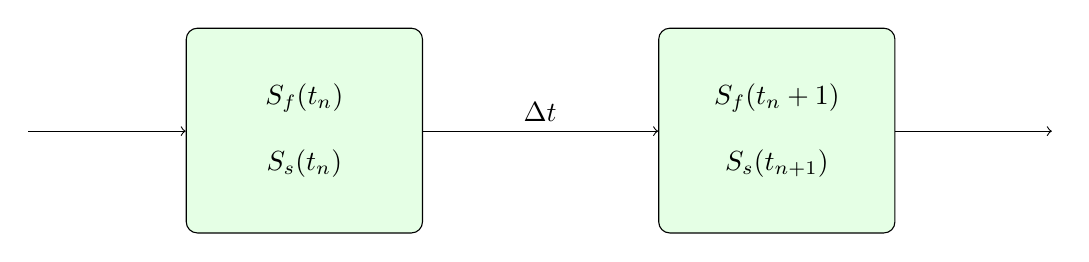
\begin{tikzpicture}[scale=1]


	\tikzstyle{status}=[draw,rectangle,rounded corners,fill=green!10,text centered,inner sep=10pt, anchor=south west, minimum width=3cm,minimum height=2.6cm]
	\draw[->] (0,1.3)-- (2,1.3) node[] {};
	
	\draw[->] (5,1.3)-- (8,1.3) node[midway,above] {$\Delta t$}; % node[midway,below] {step};

	\draw[->] (11,1.3)-- (13,1.3) node[] {};

	\node[status] (t1) at (2,0)  {
		\begin{tabular}{c}
			$S_f(t_n)$ \\
			\\
			$S_s(t_n)$
	\end{tabular}};

	\node[status] at (8,0) {
	\begin{tabular}{c}
		$S_f(t_{n}+1)$ \\
		\\
		$S_s(t_{n+1})$
\end{tabular}};
	
%		\draw (0,1.3) node[below] {$B$} --
%		(3,1.3) node[below] {$C$} --
%		(1.5,4.3) node[above] {$A$} -- cycle;
%		\draw (1.5,4.3) -- (1.5,1.3) node[below] {$D$};
%		\draw (1.5,1.5) -- (1.7,1.5) -- (1.7,1.3);
%		\node[draw,text width=3cm] at (4.5,4) {some text spanning three lines with automatic line breaks};
%		\draw[rounded corners=5pt] (4,0) rectangle ++(2,1);
	\end{tikzpicture}
	\caption{monolithic approach: $S_f$, $S_s$ denote the fluid and the structure solutions}
	\label{fig:monolithic}
\end{figure}


On the other hand, in the \textit{partitioned approach}, the fluid and the solid domains are treated as two distinct computational fields, with their respective meshes, that have to be solved separately (see Figure \ref{fig:partitioned}: how data are passed between solvers is detailed in Section \ref{sec:coupling}). The interface conditions are used explicitly to communicate information between the fluid and structure solutions. This implies that the flow does not change while the solution of the structural equations is calculated and vice versa \cite{degroote2009performance}. The partitioned approach thus requires a third software module (i.e. a coupling algorithm) to incorporate the interaction aspects. It communicates the boundary conditions described in Section \ref{sec:interface}: that is forces or stresses (dynamic data) calculated by the fluid solver at the wet surface are passed to the solid component and displacements or velocities (kinematic data) computed by the solid solver at the interface are sent to the fluid component in return. Finally, fluid and structural solutions together yield the FSI solution.

\begin{figure}[htbp!]
	\centering
	\begin{tikzpicture}[scale=1]

	\tikzstyle{solver}=[draw,rectangle,rounded corners,text centered,inner sep=10pt, anchor=south west, minimum width=3cm,minimum height=1.2cm]
	\tikzstyle{coupling}=[draw, ellipse, fill=yellow!75, minimum width=3cm, minimum height=1.2cm, align=center]

	\node[solver,fill=blue!20] at (2,4.4) {$S_f(t_n)$};
	\node[solver,fill=blue!20] at (8,4.4) {$S_f(t_{n+1})$};
	
	\node[solver,fill=orange!50] at (2,0) {$S_s(t_n)$};
	\node[solver,fill=orange!50] at (8,0) {$S_s(t_{n+1})$};
	
	\draw[->] (0,0.6)-- (2,0.6) node[] {};
	\draw[->] (5,0.6)-- (8,0.6) node[midway,above] {$\Delta t$}; % node[midway,below] {step};
	\draw[->] (11,0.6)-- (13,0.6) node[] {};


	\draw[->] (0,5)-- (2,5) node[] {};
	\draw[->] (5,5)-- (8,5) node[midway,above] {$\Delta t$}; % node[midway,below] {step};
	\draw[->] (11,5)-- (13,5) node[] {};
	
	\node[draw,fill=yellow!50,ellipse,minimum width=3cm, minimum height=1cm] at (3.5,2.8) {coupling};
	\node[draw,fill=yellow!50,ellipse,minimum width=3cm, minimum height=1cm] at (9.5,2.8) {coupling};

	\draw[->] (3,1.2)-- (3,2.3) node[midway,left] {$\vec{v}$};
	\draw[->] (4,2.3)-- (4,1.2) node[midway,right] {$\bm{\sigma}$};

	\draw[->] (3,3.3)-- (3,4.4) node[midway,left] {$\vec{v}$};
	\draw[->] (4,4.4)-- (4,3.3) node[midway,right] {$\bm{\sigma}$};

	\draw[->] (9,1.2)-- (9,2.3) node[midway,left] {$\vec{v}$};
	\draw[->] (10,2.3)-- (10,1.2) node[midway,right] {$\bm{\sigma}$};

	\draw[->] (9,3.3)-- (9,4.4) node[midway,left] {$\vec{v}$};
	\draw[->] (10,4.4)-- (10,3.3) node[midway,right] {$\bm{\sigma}$};
		
	\end{tikzpicture}
	\caption{partitioned approach: $S_f$, $S_s$ denote the fluid and the structure solutions, while $\bm{\sigma}$ and $\vec{v}$ represent coupling data}
	\label{fig:partitioned}
\end{figure}

A big advantage of this approach is that software modularity is preserved: different and efficient solution techniques can be used for the flow equations and structural equations. Provided that they can exchange data, existing solvers for the fluid and solid problem can be reused, ranging from commercial to academic and open-source codes. Those solvers are usually well-validated.
Besides, compared to monolithic procedures, the programming efforts are lower for partitioned approaches, as only the coupling of the existing solvers has to be implemented rather than the solvers themselves.
The challenge of this approach is, however, to define and implement algorithms to achieve accurate and efficient fluid-structure interaction solution with minimal code modification. Particularly, the interface
location that divides the fluid and the structure domains changes in time. The partitioned approach requires that the fluid solver has ALE capabilities, as introduced in Section \ref{subsec:ALE}.
More detailed and practical explanations about the coupling component used in this work are given in Section \ref{sec:precice}. 


\section{Coupling Strategies}
\label{sec:coupling}

Because of the modularity, the partitioned approach has gained much attention in research. The structure sketched in Figure \ref{fig:partitioned} needs to be detailed and specialized in function of the coupling strategies.

In an interface multi-physics coupling like FSI, the boundary surface is in common between the two sides of the simulation. The results make sense and are numerically stable only if the two sides of the interface are in agreement, since the output values of the one simulation become input values for the other (and vice-versa).
The solution strategies can be roughly divided into weakly and strongly coupled approaches. They are often referred to as \textit{explicit} and \textit{implicit} methods in the literature.
When the fluid and solid solutions are computed iteratively until some convergence criteria within the same time step, the scheme is called \textit{implicit coupling}. The faster, simpler but less precise \textit{explicit coupling} consists in executing a fixed number of iterations (typically one per time step) and exchange coupling values without convergence checks. 

\subsection{Explicit coupling schemes}

As in the previous Section, $S_f$ represents the fluid solver, which computes the pressures (named $d_f$ here) at the deformable boundary and $S_s$ is the structure solver, which uses these forces to compute the displacement and velocity of the boundary (named $d_s$). In a \textit{serial-explicit} (or \textit{conventional staggered}) coupling scheme, the solver $S_f$ uses the old time step boundary values $d_s^{(n)}$ to compute the values of $d_f^{(n+1)}$ for the next time step:

\begin{equation}
	d_f^{(n+1)} = S_f\left(d_s^{(n)}\right)
	\label{eq:stag1}
\end{equation}

When the fluid solver completes the time step, data are passed to the structural solver:

\begin{equation}
	d_s^{(n+1)} = S_s\left( d_f^{(n+1)} \right)
	\label{eq:stag2}
\end{equation}

Note that Equation \ref{eq:stag1} uses values computed at $t^n$, while Equation \ref{eq:stag2} uses values computed at $t^{(n+1)}$. The order of execution might be inverted.

In order reduce execution time, the solvers might run in parallel, using data from the same time step (\textit{parallel-explicit coupling}:

\begin{subequations}
\begin{eqnarray}
	d_f^{(n+1)} &=& S_f\left(d_s^{(n)}\right) \\
	d_s^{(n+1)} &=& S_s\left( d_f^{(n)} \right)
	\label{eq:par-exp}
\end{eqnarray} 
\end{subequations}


The two explicit schemes are shown schematically in Figures \ref{fig:serial-explicit} and \ref{fig:parallel-explicit}.

\begin{figure}[htbp!]
	\centering
	\begin{subfigure}{.8\textwidth}
	\centering
	% include first image
		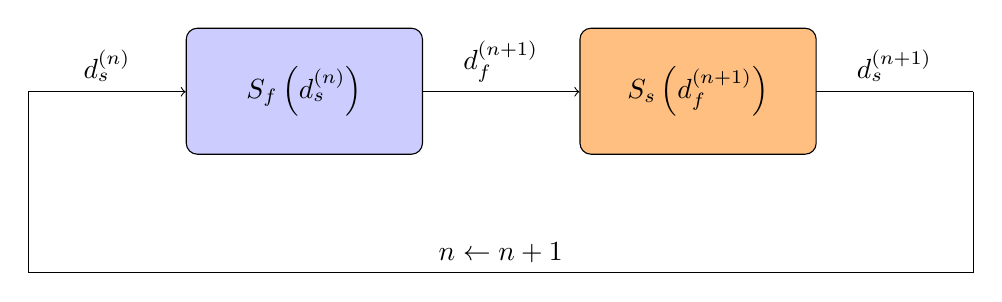
\begin{tikzpicture}[scale=1]
		\tikzstyle{solver}=[draw,rectangle,rounded corners,text centered,inner sep=10pt, anchor=south west, minimum width=3cm,minimum height=1.6cm]
		
		\node[solver,fill=blue!20] at (3,5) {$S_f\left( d_s^{(n)} \right)$};
		\node[solver,fill=orange!50] at (8,5) {$S_s\left(d_f^{(n+1)}\right)$};
		
		\draw[->] (1,5.8)-- (3,5.8) node[midway,above] {$d_s^{(n)}$};
		\draw[->] (6,5.8)-- (8,5.8) node[midway,above] {$d_f^{(n+1)}$};
		\draw[-] (11,5.8)-- (13,5.8) node[midway,above] {$d_s^{(n+1)}$};
		
		\draw[-] (13,5.8)-- (13,3.5);
		\draw[-] (1,5.8)-- (1,3.5);
		
		\draw[-] (1,3.5)-- (13,3.5) node[midway,above] {$n \leftarrow n+1$};
		
		\end{tikzpicture}
		\caption{serial explicit coupling}
		\label{fig:serial-explicit}
	\end{subfigure}
	\newline
	\centering
	\begin{subfigure}{.8\textwidth}
	\centering
	% include second image
		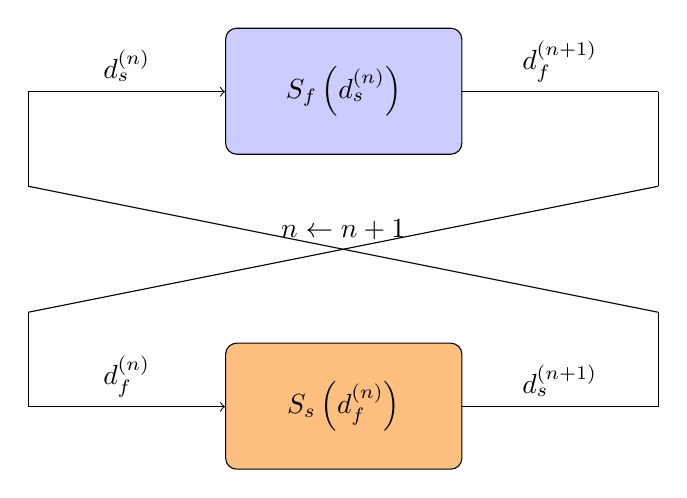
\begin{tikzpicture}[scale=1]
		\tikzstyle{solver}=[draw,rectangle,rounded corners,text centered,inner sep=10pt, anchor=south west, minimum width=3cm,minimum height=1.6cm]

		\node[solver,fill=blue!20] at (2.5,4) {$S_f\left( d_s^{(n)} \right)$};
		\node[solver,fill=orange!50] at (2.5,0) {$S_s\left(d_f^{(n)}\right)$};
		
		\draw[->] (0,4.8)-- (2.5,4.8) node[midway,above] {$d_s^{(n)}$};
		\draw[->] (0,0.8)-- (2.5,0.8) node[midway,above] {$d_f^{(n)}$};

		\draw[-] (5.5,4.8)-- (8,4.8) node[midway,above] {$d_f^{(n+1)}$};
		\draw[-] (5.5,0.8)-- (8,0.8) node[midway,above] {$d_s^{(n+1)}$};
		
		\draw[-] (0,0.8)-- (0,2);
		\draw[-] (8,0.8)-- (8,2);
		
		\draw[-] (0,3.6)-- (0,4.8);
		\draw[-] (8,3.6)-- (8,4.8);
		
		\draw[-] (8,3.6)-- (0,2) node[midway,above] {$n \leftarrow n+1$};
		\draw[-] (0,3.6)-- (8,2);

	
		\end{tikzpicture}
		\caption{parallel explicit coupling}
		\label{fig:parallel-explicit}
	\end{subfigure}
	\caption{Explicit coupling schemes}
\end{figure}

In general, an explicit coupling is not enough to regain the exact (as in the monolithic approach) solution of the problem as the matching coupling conditions between the solvers is not enforced within each time step: no balance between fluid and structural domain with respect to forces and displacements at the interface can be guaranteed (\cite{hou2012numerical}, \cite{degroote2009performance}). Nevertheless, explicit coupling yields good results if the interaction between fluid and solid is weak as in aeroelastic simulations, where in general the simulations show small displacements of the structure within a single time step and the flow field isn't much influenced by the structural displacements (\cite{farhat2006provably}).

\subsection{Implicit coupling schemes}


On the other hand, strongly (implicit) coupling techniques require an iterative method to solve the fixed-point equation that derives from enforcing the agreement of the interface variables.
The coupling conditions at the wet surface are enforced in each time step up to a convergence criterion. If the criterion is not met, another subiteration within the same time instance is computed. Therefore, the solution can approximate the monolithic solution to an arbitrary accuracy.

As in the explicit case, solvers may run in a sequential mode: the coupling is then named \textit{serial} (or staggered) and the solvers wait for each other. 

\begin{subequations}
	\begin{eqnarray}
		d_f^{(n+1),i+1} &=& S_f\left(d_s^{(n+1),i}\right) \\
		d_s^{(n+1),i+1} &=& S_s\left( d_f^{(n+1),i+1} \right)
	\end{eqnarray} 
	\label{eq:ser-imp}
\end{subequations}

Equations \ref{eq:ser-imp} show that, in contrast with explicit coupling, both solvers use interface values at time step $n+1$, but one of them uses data from previous iteration.
If run in parallel mode \cite{mehl2016parallel}, the system becomes:

\begin{subequations}
	\begin{eqnarray}
		d_f^{(n+1),i+1} &=& S_f\left(d_s^{(n+1),i}\right) \\
		d_s^{(n+1),i+1} &=& S_s\left( d_f^{(n+1),i} \right)
	\end{eqnarray} 
	\label{eq:par-imp}
\end{subequations}

At convergence, the following relation holds of serial (or \textit{Gauss-Seidel}) coupling:


\begin{subequations}
	\begin{eqnarray}
		d_s^{(n+1)} &=&  S_s\left(S_f\left(d_s^{(n+1)}\right) \right) \\
		\label{eq:ser-fp-comp}
		d_s^{(n+1)} &=& S_s  \circ S_f \left( d_s^{(n+1)} \right)
	\end{eqnarray} 
	\label{eq:ser-fp}
\end{subequations}


and the following relation holds for parallel (or \textit{Jacobi}) coupling:

\begin{equation}
	\begin{pmatrix}
		d_s^{(n+1)} \\
		d_f^{(n+1)}
	\end{pmatrix} = 
	\begin{pmatrix}
		0 & S_f \\
		S_s & 0
	\end{pmatrix} 
	\begin{pmatrix}
		d_s^{(n+1)} \\
		d_f^{(n+1)}
	\end{pmatrix}
	\label{eq:par-fp}
\end{equation}


Acceleration techniques are necessary to bring fixed point equation \ref{eq:ser-fp-comp} or \ref{eq:par-fp} to convergence. Those techniques are described in Section \ref{sec:strong-coupling}.

The two implicit schemes are shown schematically in Figures \ref{fig:serial-implicit} and \ref{fig:parallel-implicit}: \textit{accel} refers to the post-processing step implemented to speedup convergence. After every non-converged iteration, the latest stored state of the solver (\textit{checkpoint}) is reloaded and coupling iteration \textit{i} for the current time step is incremented. When the solution converges, the time step \textit{n} is incremented.


\begin{figure}[htbp!]
	\centering
	\begin{subfigure}{.8\textwidth}
		\centering
		% include first image
		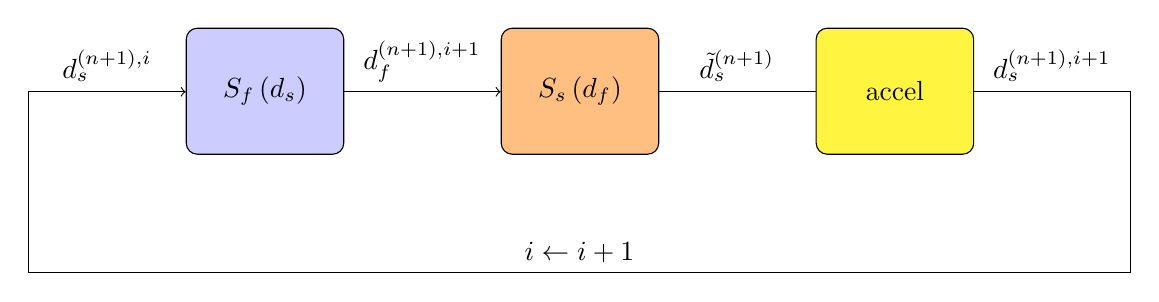
\begin{tikzpicture}[scale=1]
			\tikzstyle{solver}=[draw,rectangle,rounded corners,text centered,inner sep=10pt, anchor=south west, minimum width=2cm,minimum height=1.6cm]
			
			\node[solver,fill=blue!20] at (2,5) {$S_f\left( d_s\right)$};
			\node[solver,fill=orange!50] at (6,5) {$S_s\left(d_f\right)$};
			\node[solver,fill=yellow!75] at (10,5) {accel};
			
			\draw[->] (0,5.8)-- (2,5.8) node[midway,above] {$d_s^{(n+1),i}$};
			\draw[->] (4,5.8)-- (6,5.8) node[midway,above] {$d_f^{(n+1),i+1}$};
			\draw[-] (8,5.8)-- (10,5.8) node[midway,above] {$\tilde{d}_s^{(n+1)}$};
			\draw[-] (12,5.8)-- (14,5.8) node[midway,above] {$d_s^{(n+1),i+1}$};
			
			\draw[-] (14,5.8)-- (14,3.5);
			\draw[-] (0,5.8)-- (0,3.5);
			
			\draw[-] (0,3.5)-- (14,3.5) node[midway,above] {$i \leftarrow i+1$};
			
		\end{tikzpicture}
		\caption{serial implicit coupling}
		\label{fig:serial-implicit}
	\end{subfigure}
	\newline
	\centering
	\begin{subfigure}{.8\textwidth}
		\centering
		% include second image
		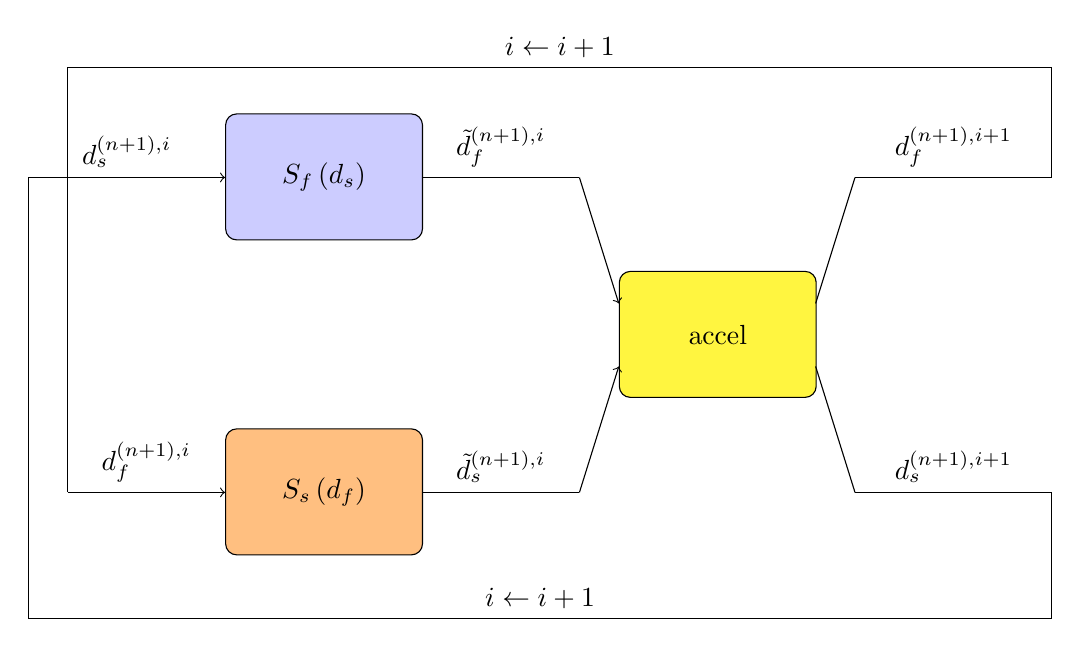
\begin{tikzpicture}[scale=1]
			\tikzstyle{solver}=[draw,rectangle,rounded corners,text centered,inner sep=10pt, anchor=south west, minimum width=2.5cm,minimum height=1.6cm]
			
			\node[solver,fill=blue!20] at (2.5,4) {$S_f\left( d_s \right)$};
			\node[solver,fill=orange!50] at (2.5,0) {$S_s\left(d_f\right)$};
			
			\node[solver,fill=yellow!75] at (7.5,2) {accel};
			
			\draw[->] (0,4.8)-- (2.5,4.8) node[midway,above] {$d_s^{(n+1),i}$};
			\draw[->] (0.5,0.8)-- (2.5,0.8) node[midway,above] {$d_f^{(n+1),i}$};
			
			\draw[-] (5,4.8)-- (7,4.8) node[midway,above] {$\tilde{d}_f^{(n+1),i}$};
			\draw[-] (5,0.8)-- (7,0.8) node[midway,above] {$\tilde{d}_s^{(n+1),i}$};
			
			\draw[->] (7,4.8)-- (7.5,3.2);
			\draw[->] (7,0.8)-- (7.5,2.4);
			
			\draw[-] (10,3.2)-- (10.5,4.8);
			\draw[-] (10,2.4)-- (10.5,0.8);

			\draw[-] (10.5,4.8)-- (13,4.8) node[midway,above] {$d_f^{(n+1),i+1}$};
			\draw[-] (10.5,0.8)-- (13,0.8) node[midway,above] {$d_s^{(n+1),i+1}$};

			\draw[-] (13,4.8)-- (13,6.2);
			\draw[-] (13,0.8)-- (13,-0.8);

			\draw[-] (13,6.2)-- (0.5,6.2) node[midway,above] {$i \leftarrow i+1$};
			\draw[-] (13,-0.8)-- (0,-0.8) node[midway,above] {$i \leftarrow i+1$};
			
			\draw[-] (0,-0.8)-- (0,4.8);
			\draw[-] (0.5,6.2)-- (0.5,0.8);

			%\draw[-] (0,0.8)-- (0,2);
			%\draw[-] (8,0.8)-- (8,2);
			
			%\draw[-] (0,3.6)-- (0,4.8);
			%\draw[-] (8,3.6)-- (8,4.8);
			
			%\draw[-] (8,3.6)-- (0,2) node[midway,above] {$n \rightarrow n+1$};
			%\draw[-] (0,3.6)-- (8,2);
			
			
		\end{tikzpicture}
		\caption{parallel implicit coupling}
		\label{fig:parallel-implicit}
	\end{subfigure}
	\caption{Implicit coupling schemes}
\end{figure}

Implicit methods are generally applicable to any kind of FSI problems, in contrast with explicit methods. When fluid and structure are strongly coupled, explicit coupling can be subject to numerical instabilities, a problem that cannot always be solved by reducing the coupling time step size \cite{van2009added}. These instabilities can be overcome by implicit methods, even if several coupling iterations may be executed every time step, until the values on both sides of the interface converge.


\section{Strong coupling algorithms}
\label{sec:strong-coupling}

As mentioned in the previous section, implicit methods require some post-processing (generally called \textit{acceleration}) techniques to to make the solution of the single time step of the coupled partitioned FSI problem converge. This requires to solve a a \textit{fixed-point equation}, in fact:

\begin{subequations}
	\begin{eqnarray}
		\label{eq:fp-def}
		H(d_s) &\coloneqq&  S_s  \circ S_f(d_s)  \\
		\label{eq:fp-2}
		d_s &=& H(d_s)  \\
		\label{eq:fp3}
		R(d) &\coloneqq& H(d) - d = 0
	\end{eqnarray} 
	\label{eq:fp-equations}
\end{subequations}

Equation \ref{eq:fp-def} represents the composition of the solid and the fluid solution, while Equation \ref{eq:fp-2} represents the resulting fixed point equation. As the order of execution can be switched, in Equation \ref{eq:fp3}, where the \textit{residual} is defined, the input data $d_s$ is generically substituted with $d$.

The basic approach to solve the fixed point equation is to perform the corresponding ~\ac{FPI}:

\begin{equation}
	x_{i+1} = H(x_i) \quad i=1,2,\ldots
\end{equation} 

which is known to converge if the mapping \textit{H} is a contraction, but this is not the general case in FSI computations \cite{mehl2016parallel}. 

\subsection{under-relaxation}

The way to stabilize the iterations is to perform a FPI with \textit{under-relaxation} as illustrated in the following algorithm:

\begin{algorithm}[H]
	\SetAlgoLined
	\KwResult{$d_k$}
	initialization of $d_0$\;
	k = 0\;
	$\tilde{d}_1 = S_s \circ S_f(d_0)$\;
	$r_0$ = $\tilde{d}_1 - d_0$\;
	\While{$\lVert r_k \rVert > \varepsilon$}{
		compute $d_k$ by relaxation\;
		k = k +1\;
	}
	\caption{FPI with relaxation}
\end{algorithm}

The under-relaxation is defined by:

\begin{equation}
	d_{k+1} = d_{k} + \omega \left( H(d_k)  - d_k  \right)
	\label{eq:ur}
\end{equation} 

Where $\omega$ in Equation \ref{eq:ur} is the \textit{relaxation factor}. The relaxation parameter has to be small enough to keep the iteration from diverging, but as large as possible in order to use as much of the new solution as possible \cite{kuttler2008fixed}. The optimal $\omega$ value is problem specific and not known a priori.
A suitable dynamic relaxation parameter, is a better choice, like the \textit{Aitken under-relaxation} \cite{irons1969version} which adapts the factor at each iteration with the following relation:

\begin{equation}
	\omega_i = -\omega_{i-1} \frac{r_{i-1}^T \left(r_i - r_{i-1}\right)}{ \lVert r_i - r_{i-1} \rVert ^2}
\end{equation}

Aitken under-relaxation can be a good choice for strong interaction with a fluid solvers that does not fully converge in every iteration or for compressible fluid solvers.


\subsection{Quasi Newton Least Squares schemes}

Under-relaxation is a good choice for easy stable problems, but is outperformed by more sophisticated quasi-Newton coupling schemes. Equation \ref{eq:fp3} could be solved iteratively with a Newton method \cite{uekermann2016partitioned}:

\begin{subequations}
	\begin{eqnarray}
		\label{eq:nm1}
		R(d_k) &\coloneqq&  r_k  \\
		\label{eq:nm2}
		R(d_k) + \left. \frac{\partial R}{\partial d}\right|_{d_k} \left( d_{k+1} - d_k \right) &=& 0 \\
		\label{eq:nm3}
		d_k + \left(  \left. \frac{\partial R}{\partial d} \right|_{d_k} \right)^{-1} \left(-r_k \right) &=&  d_{k+1}
	\end{eqnarray} 
	\label{eq:fp-jac}
\end{subequations}

The \textit{residual} at iteration \textit{k} is defined in Equation \ref{eq:nm1}, if the Jacobian matrix of the equation is known, a Newton iteration can be performed as in Equation \ref{eq:nm2}. The updated values can be computed using Equation \ref{eq:nm3}.

In situations where:
\begin{itemize}
	\item \textit{black-box} systems are considered (i.e. the Jacobian is unknown),
	\item the cost of a function evaluation is sufficiently high that numerical estimation of the Jacobian is prohibitive, 
\end{itemize}

there exist a number of matrix-free methods that use only information derived from the consecutive iterates and that build an approximation based on those values. This approach is known as \textit{quasi-Newton method} \cite{haelterman2009quasi}.
Input and output data of $H$ and $R$ are used to approximate the solution of \ref{eq:nm3}. Algorithm \ref{alg:qnls} (taken from \cite{uekermann2013parallel}) shows the basics steps to estimate data at next step using the \textit{Quasi Newton Least Squares Method}:

\begin{algorithm}[H]
	\SetAlgoLined
	\KwResult{$d_{k+1}$}
	initial value $d_0$\;
	$\tilde{d}_0 = H(d_0)$ and $R_0 = \tilde{d}_0 +- d_0$\;
	$d_1 = d_0 + \omega r_0$\;
	\For{$k = 1 \ldots$}{
		$\tilde{d}_k = H(d_k)$ and $r^k = \tilde{d}_k - d_k$\;
		$V^k = \left[\Delta r_0^k, \ldots , \Delta r^k_{k-1} \right]$ with $\Delta r^k_i =r^i - r^k$\;
		$W^k = \left[\Delta \tilde{d}^k_0, \ldots , \Delta \tilde{d}^k_{k-1}  \right]$ with $\Delta \tilde{d}^k_i = \tilde{d}_i - d_k$\;
		decompose $V^k = Q^kU^k$\;
		solve the first $k$ lines of $U^k \alpha = - Q^{k^T}R^k$\;
		$\Delta \tilde{d}^k = W^k\alpha$\;
		$d_{k+1} = \tilde{d}_k + \Delta \tilde{d}_k$\;
		
	}
	\label{alg:qnls}
	\caption{Quasi Newton Least Squares method}
\end{algorithm}

In algorithm \ref{alg:qnls} the matrices $V^k$ and $W^k$ are constructed from the previous iterations and the known values of $d_0, \ldots d_k$ and $\tilde{d}_0, \ldots, \tilde{d}_k$. $\Delta \tilde{d}^k$ is constructed in the column space of $W^k$ (line 10). For this reason a least squares problem is solved:

\begin{equation}
	\alpha = \argmin_{\beta \in \mathbb{R}^k} \lVert V^k\beta + R(d_k) \rVert
\end{equation}

The least squares problem is solved  computing the decomposition of $V^k$ into an orthogonal matrix $Q^k \in \mathbb{R}^{k \times k} $ and an upper triangular matrix $U^k \in \mathbb{R}^{n \times k}$ (line 8). Then $\alpha$ is computed in line 9.

When building matrices $V^k$ and $W^k$ (lines 6-7 ), it is possible to use information from previous time steps.

Finally, to ensure linear independence of columns in the multi-secant system for Jacobian estimation, a filter can be used \cite{haelterman2016improving}, in order to drop nearly dependent columns of $Q^k$ and avoid singularity of the approximated Jacobian.

The above algorithm is usually denominated in FSI  ~\ac{IQN-ILS} (or Anderson acceleration). There exist other algorithms, like generalized Broyden (IQN-IMVJ) or manifold mapping to solve the problem. A complete desciption of those methods goes beyond the scope of this work: a description of the most common algorithms can be found in \cite{blom2016review}, while a comparison of the performances can be found in \cite{lindner2015comparison}.


\subsection{Convergence criteria}

At each time step, the coupling algorithm enforce matching conditions at the wet surface up to a convergence criterion. If not sufficiently met, another iteration within the same time step is performed. The fixed point formulation itself induces a criterion based on the residual itself $r_{k+1}$.

A scalar, \textit{absolute convergence criterion} can de defined as in Equation \ref{eq:abscrit}: it is useful for close to zero values of the coupling quantities, when rounding errors become important:

\begin{equation}
	\lVert r_{k+1} \rVert \leq \epsilon_{abs}
	\label{eq:abscrit}
\end{equation}

A more common \textit{relative convergence criterion}, defined in Equation \ref{eq:relcrit} is particularly useful when different quantities (e.g. forces and displacements) are compared together to evaluate convergence:


\begin{equation}
	\frac{\lVert  r_{k+1} \rVert}{\lVert  \tilde{d}_{k+1} \rVert} \leq \epsilon_{rel}
	\label{eq:relcrit}
\end{equation}



\section{Interface Mesh and Data Mapping}
\label{sec:interface-mesh}

FSI methods can also be classified considering how the fluid and solid meshes are treated. The \textit{conforming mesh methods} consider the interface as a physical boundary condition (see Section \ref{sec:conforming-mesh}), while \textit{non-conforming mesh methods} treat the boundary location as a constraint imposed on the model equations (see Section \ref{sec:nonconforming-mesh}) \cite{hou2012numerical}.


\subsection{Non-conforming Mesh methods}
\label{sec:nonconforming-mesh}

In non-conforming mesh strategies all interface conditions are imposed as constraints on the flow and structural governing equations. It is possible to use non-conforming meshes for fluid and solid domains as they remain geometrically independent from each other (see Figure \ref{fig:nonconf-mesh}).

This approach is mostly used in \textit{immersed boundary} methods \cite{kajishima2017immersed}. Coupling is imposed by means of additional force terms appearing in the model equations of the fluid, which impose the kinematic and dynamic conditions.
The forces represent the effects of a boundary or body being immersed in the fluid domain. A purely Eulerian mesh (see Section \ref{subsec:euler}) can be used for the whole computational domain, since
the force terms are dynamically added at specific locations to represent the structure.

The fluid forces applied on the solid at the wet surface are computed and used as input for the structural solver, which employs a standard Lagrangian mesh (see Section \ref{subsec:lagrange}).

Immersed boundary methods are particularly innovative and are useful to overcome some issues in CFD computations, on the other hand most of the current implementations of FSI problem implement a conforming mesh strategy.

\begin{figure}[htbp!]
	\centering
	\begin{subfigure}{.5\textwidth}
		\centering
		\includegraphics[width=.9\linewidth]{images/nonconf1c}
		\caption{mesh at $t=t_1$}
		\label{fig:nc1}
	\end{subfigure}%
	\begin{subfigure}{.5\textwidth}
		\centering
		\includegraphics[width=.9\linewidth]{images/nonconf2c}
		\caption{mesh at $t=t_2$}
		\label{fig:nc2}
	\end{subfigure}
	\caption{non conforming mesh example}
	\label{fig:nonconf-mesh}
\end{figure}


\subsection{Conforming Mesh methods}
\label{sec:conforming-mesh}

Conforming mesh methods adapt very well to the partitioned approach described in Section \ref{sec:monolithic} as they usually consists in the computational steps described above, namely: computation in the fluid, computation in the solid, enforcing of interface condition and mesh movement (see Figure \ref{fig:conf-mesh}).   

Fluid and structure meshes need share the boundary of the wet surface, as the coupling conditions are enforced by applying kinematic or dynamic conditions to those boundaries.
Node-to-node matching of fluid and structure meshes at the interface is not required, as long as a suitable mapping between the interface nodes is performed (see Section \ref{sec:data-mapping}).

The match between the interfaces must hold at each time step: this implies that both solid and fluid domains need to deform. Deformation is easily expressed in the solid domain as the structural mesh is usually represented in Lagrangian perspective (see Section \ref{subsec:lagrange}). ALE perspective (Section \ref{subsec:ALE}) for the fluid domain becomes necessary in this case.

Mesh deformation can turn out to be a complicated task as in general the fluid mesh is deformed during motion (see Figure \ref{fig:ale-mesh}). Mesh smoothing techniques need to be applied in order to keep a good mesh quality in terms of distorted elements which can lead to accuracy loss in simulations. (the following video shows high distorted fluid elements during FSI motion: \href{https://youtu.be/zJ7PR90Y2TI}{video}). 

Mesh smoothing is generally applied to keep the fluid mesh as uniform and undistorted as possible during movement.
There is a wide variety of mesh updating procedures \cite{van2007comparison}.
The \textit{torsional spring analogy} \cite{degand2002three} is a fairly simple technique that computes mesh movement considering mesh edges as springs and solving the subsequent Laplace equation that derives from the mesh movement. 

Some other references about mesh motion alternatives can be found in \cite{gonzalez2009mesh}.


\begin{figure}[htbp!]
	\centering
	\begin{subfigure}{.5\textwidth}
		\centering
		\includegraphics[width=.9\linewidth]{images/conf1c}
		\caption{mesh at $t=t_1$}
		\label{fig:c1}
	\end{subfigure}%
	\begin{subfigure}{.5\textwidth}
		\centering
		\includegraphics[width=.9\linewidth]{images/conf2c}
		\caption{mesh at $t=t_2$}
		\label{fig:c2}
	\end{subfigure}
	\caption{conforming mesh example}
	\label{fig:conf-mesh}
\end{figure}



\subsection{Data Mapping}
\label{sec:data-mapping}

When partitioned coupling is involved and the meshes are conforming but not node-to-node coincident, the challenge is to correctly map the data between the solid and the fluid sides. This is a common situation as fluid and solid require a different mesh refinement at the interface.

The mapping procedure needs not only to find the closest available mesh point (or points) on the opposite mesh, but also to preserve mass and energy balance. Variables are basically mapped in two ways: \textit{consistent} and \textit{conservative} forms.

In the \textit{consistent mapping} a value on a node of one grid has the same value of the corresponding node on another grid: that is, it reproduces the values on both meshes. In the \textit{conservative form}, integral values are preserved between meshes. In an FSI problem, nodal forces are mapped in conservative form, while velocities or displacements are mapped in consistent form. An example is shown in Figure \ref{fig:mapping}.



\begin{figure}[htbp!]
	\centering
	\begin{subfigure}{.8\textwidth}
		\centering
		% include first image
		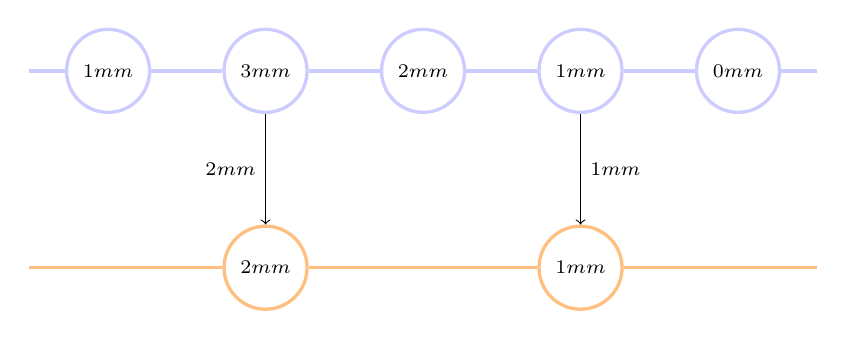
\begin{tikzpicture}[scale=1]
			\tikzstyle{n} = [draw, very thick, circle, minimum width=30]
			\node [n,draw=blue!20] (f1) at (1,2.5) {\scriptsize{$1mm$}};
			\node [n,draw=blue!20] (f2) at (3,2.5) {\scriptsize{$3mm$}};
			\node [n,draw=blue!20] (f3) at (5,2.5) {\scriptsize{$2mm$}};
			\node [n,draw=blue!20] (f4) at (7,2.5) {\scriptsize{$1mm$}};
			\node [n,draw=blue!20] (f5) at (9,2.5) {\scriptsize{$0mm$}};
			\node [n,draw=orange!50] (s1) at (3,0) {\scriptsize{$2mm$}};
			\node [n,draw=orange!50] (s2) at (7,0) {\scriptsize{$1mm$}};
			
			\draw [very thick, blue!20] (0,2.5) -- (f1);
			\draw [very thick, blue!20] (f1) -- (f2);
			\draw [very thick, blue!20] (f2) -- (f3);
			\draw [very thick, blue!20] (f3) -- (f4);
			\draw [very thick, blue!20] (f4) -- (f5);
			\draw [very thick, blue!20] (f5) -- (10,2.5);
			
			\draw [very thick, orange!50] (0,0) -- (s1);
			\draw [very thick, orange!50] (s1) -- (s2);
			\draw [very thick, orange!50] (s2) -- (10,0);
			
			\draw[->] (f2)-- (s1) node[midway,left] {\scriptsize{$2mm$}};
			\draw[->] (f4)-- (s2) node[midway,right] {\scriptsize{$1mm$}};
			
		\end{tikzpicture}
		\caption{consistent mapping}
		\label{fig:consistent}
	\end{subfigure}
	\newline
	\centering
	\begin{subfigure}{.8\textwidth}
		\centering
		% include second image
		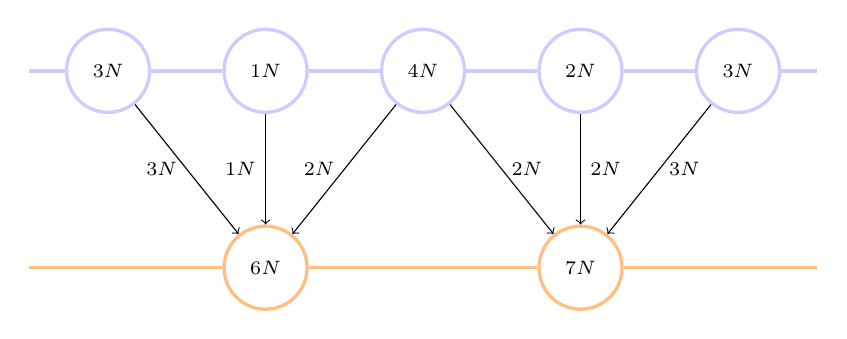
\begin{tikzpicture}[scale=1]
			\tikzstyle{n} = [draw, very thick, circle, minimum width=30]
			\node [n,draw=blue!20] (f1) at (1,2.5) {\scriptsize{$3N$}};
			\node [n,draw=blue!20] (f2) at (3,2.5) {\scriptsize{$1N$}};
			\node [n,draw=blue!20] (f3) at (5,2.5) {\scriptsize{$4N$}};
			\node [n,draw=blue!20] (f4) at (7,2.5) {\scriptsize{$2N$}};
			\node [n,draw=blue!20] (f5) at (9,2.5) {\scriptsize{$3N$}};
			\node [n,draw=orange!50] (s1) at (3,0) {\scriptsize{$6N$}};
			\node [n,draw=orange!50] (s2) at (7,0) {\scriptsize{$7N$}};

			\draw [very thick, blue!20] (0,2.5) -- (f1);
			\draw [very thick, blue!20] (f1) -- (f2);
			\draw [very thick, blue!20] (f2) -- (f3);
			\draw [very thick, blue!20] (f3) -- (f4);
			\draw [very thick, blue!20] (f4) -- (f5);
			\draw [very thick, blue!20] (f5) -- (10,2.5);

			\draw [very thick, orange!50] (0,0) -- (s1);
			\draw [very thick, orange!50] (s1) -- (s2);
			\draw [very thick, orange!50] (s2) -- (10,0);

			\draw[->] (f1)-- (s1) node[midway,left] {\scriptsize{$3N$}};
			\draw[->] (f2)-- (s1) node[midway,left] {\scriptsize{$1N$}};
			\draw[->] (f3)-- (s1) node[midway,left] {\scriptsize{$2N$}};
			\draw[->] (f3)-- (s2) node[midway,right] {\scriptsize{$2N$}};
			\draw[->] (f4)-- (s2) node[midway,right] {\scriptsize{$2N$}};
			\draw[->] (f5)-- (s2) node[midway,right] {\scriptsize{$3N$}};
			
		\end{tikzpicture}
		\caption{conservative mapping}
		\label{fig:conservative}
	\end{subfigure}
	\caption{Examples of mapping data between non-coincident meshes: consistent (a) and conservative (b) schemes.}
	\label{fig:mapping}
\end{figure}


different mapping strategies can be implemented \cite{bungartz2016precice}:

\begin{itemize}
	\item \textit{Nearest Neighbor}: finds the closest point on the source mesh and uses its value for the target mesh. It does not require any topological information and is first-order accurate. It is the computationally easiest implementation and it is useful when interface meshes are coincident.
	\item \textit{Nearest Projection}: projects the points of the target mesh on the source mesh, interpolates the data linearly and assigns the values to the target mesh. It requires topology information for the source mesh. The interpolation on the mesh elements is second order accurate.
	\item \textit{~\ac{RBF}}: this method does not requires topological information and works well on general meshes. The mapping uses radial basis functions centered at the grid points of the source mesh \cite{lindner2017radial}.
\end{itemize}


\section{Stability: Added Mass Effect}
\label{sec:added-mass}

When a solid moves or vibrates in a fluid domain, the interaction changes the way in which the structure behaves. There exist a vast variety of literature (e.g.: \cite{chen1976added}, \cite{conca1997added}, \cite{gauthier2017numerical}, \cite{ricciardi2015modelling}) describing the effects of FSI in terms of \textit{added mass}, \textit{added damping} or even \textit{added stiffness} effects on a vibrating structure in function of fluid properties (e.g. density or viscosity), or flow properties (e.g. velocity).

Besides the physical aspects of the interaction, some numerical issues arise when trying to simulate this kind of problems.

The numerical issue named \textit{~\ac{AME}} is introduced here, as it is relevant for both strongly and weakly coupled partitioned approaches in the solution of FSI problems. 

Weakly coupled algorithms give good results in aeroelasticity studies, but 


\cite{van2009added}
\cite{causin2005added}
\cite{forster2006artificial}
\cite{degroote2008stability}


As already mentioned in Section 2.3.3, there can be no gaps between structure and fluid. Also their
respective particles cannot occupy the same spatial locations simultaneously. Thus, if the solid is moved,
also fluid particles move. Changing the state of motion of the structural component consequently requires
taking into account inertial effects not only of the solid itself, but also of the surrounding fluid, which
artificially rests for the span of a single structure solver time step. In more descriptive words: Moving the
solid also implies moving fluid particles close to the solid. Therefore, the structure behaves more inert
due to artificially added mass ([42], [2]). Since inertia is dependent on mass and therefore density, the
% AME is also. More precisely, it is dependent on the ratio (MA) of structural (S) und fluid density (F )
([42], [5]):
%MA = S F : (3.1)
This ratio is often used to describe how strong the interaction between solid and fluid is. For cases, in
%which the solid density is much higher than the fluid density (MA  1), this effect does not dominantly
influence the FSI problem (weak interaction). But as fluid and structure densities approach each other
%(MA  1) or the fluid becomes even denser than the solid (MA < 1), its consideration is crucial (strong
interaction) and imposes stability limits on partitioned solution techniques ([5], [42], [2]). Note that the
AME is not only governed by the density ratio of Equation 3.1 but also by geometric properties of the
problem, the stiffness of the solid ([5]) and the speed of sound in the flow domain ([42]). Nonetheless,
for the sake of simplicity and intuitiveness, explanations in this thesis are mostly limited to the density
ratio.
In general, the AME is of bigger concern for incompressible flows than for compressible regimes. From
a physical point of view, deformations of the structural domain can be interpreted as perturbations for
the flow field. In compressible flows the speed of sound (speed at which perturbations propagate through
the flow) is finitely large. Thus, the influence of a geometrical change of the fluid domain caused by
deformations of the solid is locally limited during a certain period of time. In contrast, in incompressible
flows the speed of sound is infinitely large, hence all perturbations propagate through the flow without
time delay. Therefore, regardless of how much time has passed since a perturbation, the whole flow field
is directly affected ([42], [5]).
In the following it is assumed that a weakly coupled algorithm allows computation of the fluid and solid
solution only once per time step. In addition, coupling data is also exchanged once per time instance. In
contrast, a strongly coupled solver does the same at least twice per time increment (for a reminder see
Section 3.2 and compare Figure 3.4). As can be shown, in the compressible case a more dominant AME
can be compensated for by reducing the time step size of strongly coupled, partitioned solution algorithms.
This however, does not hold for the incompressible regime, where even in the limit of vanishing time step
size strongly coupled, partitioned algorithms might fail ([42]). These observations are consistent with the
above mentioned physical explanation.
First of all, considering compressible flows, indeed, the lack of repeated subiterations in weakly coupled
partitioned techniques leads to a strict limit for the density ratio (of Equation 3.1) due to the fact that
the interface conditions are not enforced and energy balance at the wet surface is generally not given.
If that limit is exceeded the algorithm fails due to instability ([2]). Likewise, in such a case a strongly
coupled partitioned algorithm converges slowly, resulting in possibly many necessary subiterations, which
is computationally costly. Yet it does not become unstable, given that the time step size is chosen sufficiently
small. Reducing the time step size to an arbitrarily small extent cannot stabilize a weakly coupled
approach if the stability criterion on the density ratio is not met ([15]). Conversely, the convergence
rate of strongly coupled algorithms increases by the same factor, by which the time step size decreases,
meaning that in the limit of vanishing time step size the monolithic solution is obtained ([5], [42]).
In the incompressible case however, a strict stability limit exists for both weakly and strongly coupled
algorithms. It is independent of the size of time increments1. Furthermore, in order for an implicit
method to achieve the monolithic solution (assuming its convergence is given, i.e. the before mentioned
stability limit is not exceeded) the number of subiterations must be increased as time step size decreases
([15], [42]).







To conclude this chapter about computational aspects of FSI simulations, the AME is briefly described.
Explanations of this effect can be found in a great variety throughout FSI literature, typically explicated
for specific solver strategies or flow regimes (see e.g. [5], [42], [15], [2]). Therefore, in the scope of
this thesis only a short phenomenological introduction to the concept of added mass and numerical
problems arising from it is given. However, this suffices to focus on both weakly and strongly coupled partitioned approaches, which are practically relevant in this thesis. The AME is inherent to partitioned
FSI approaches as the single-physics fields are not continuously coupled but interaction only occurs at a
finite number of discrete time instances, when coupling quantities are exchanged.